\documentclass{beamer}

% Top-aligning columns within a top-aligned frame
% https://tex.stackexchange.com/questions/16447/beamer-top-aligning-columns-within-a-top-aligned-frame
\makeatletter
\newenvironment{myitemize}{%
   \setlength{\topsep}{0pt}
   \setlength{\partopsep}{0pt}
   \renewcommand*{\@listi}{\leftmargin\leftmargini \parsep\z@ \topsep\z@ \itemsep\z@}
   \let\@listI\@listi
   \itemize
}{\enditemize}
\makeatother  

\usepackage[USenglish]{babel}
\usepackage[utf8]{inputenc}
\usepackage{amssymb, amsmath}
\usepackage{bm}
\usepackage{color}
\usepackage{tikz}
\usepackage{url}

\definecolor{links}{HTML}{2A1B81}
\hypersetup{colorlinks,linkcolor=,urlcolor=links}

\usetheme{Boadilla}

\bibliographystyle{apalike}
% make bibliography entries smaller
%\renewcommand\bibfont{\scriptsize}
% Now get rid of all the colours
\setbeamercolor*{bibliography entry title}{fg=black}
\setbeamercolor*{bibliography entry author}{fg=black}
\setbeamercolor*{bibliography entry location}{fg=black}
\setbeamercolor*{bibliography entry note}{fg=black}

\newcommand{\lnorm}[1]{\left\lVert#1\right\rVert^2}
\newcommand{\norm}[1]{\left\lVert#1\right\rVert}

% and kill the abominable icon
\setbeamertemplate{bibliography item}{}

\begin{document}
\title[DeBERTa]{DeBERTa: Decoding-enhanced BERT with Disentangled Attention}  
\author{Radek Bartyzal}
\date{2. 3. 2021} 
\institute{GLAMI AI}

\frame{\titlepage} 

%--------- END Frame 12 -------------
\begin{frame}{Motivation}

Paper is by Microsoft Research from 2020/2021.
\vfill

\begin{itemize}
\item improved BERT
\item models available through Hugging Face
\end{itemize}


\end{frame}
%--------- END Frame 12 -------------
\begin{frame}{BERT}

Transformer + 

\end{frame}
%--------- END Frame 12 -------------
\begin{frame}{DeBERTa changes to BERT}


\textbf{disentangled attention mechanism}: treat content and position information separately

\vfill

\textbf{relative positional encodings} passed to each layer

\vfill

\textbf{enhanced mask decoder}: provide absolute positional encodings only after the last layer before decoding softmax

\end{frame}
%--------- END Frame 12 -------------
\begin{frame}{Classic attention mechanism}


\begin{figure}[h]
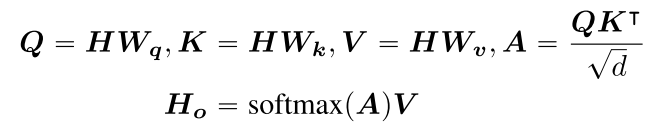
\includegraphics[width=0.6\textwidth]{img/att}
\end{figure}

\begin{itemize}
\item before the first layer word vectors are summed with positional vectors
\item these combined = entangled content vectors are then passed through Transformer layers
\item each layer's attention creates Key, Query and Value vectors from these combined vectors
\end{itemize}

\end{frame}
%--------- END Frame 12 -------------
\begin{frame}{Disentangled attention mechanism}


disentangled attention = at each layer, create separate Key and Query vectors = $K^r$ and $Q^r$ from relative positional vectors 
\begin{figure}[h]
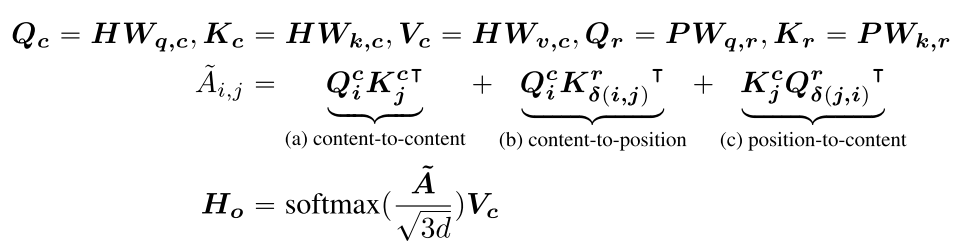
\includegraphics[width=\textwidth]{img/att2}
\end{figure}

\begin{itemize}
\item there is still only one Value vector created from content vector
\item content vectors are the ones transformed by each layer, positional vectors stay the same
\item final attention matrix is sum of attention matrices of possible combinations of Pos. and Content Q/Ks
\end{itemize}

\end{frame}
%--------- END Frame 12 -------------
\begin{frame}{Disentangled attention mechanism}

$P_{i,j}$ = encoding of a position of $i$ relative to $j$
\begin{figure}[h]
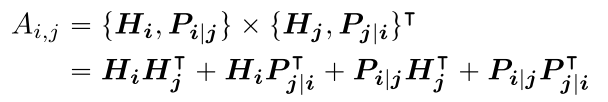
\includegraphics[width=\textwidth]{img/attij}
\end{figure}

Possible attention matrices = combinations of P, C:
\begin{itemize}
\item C to C = classic attention
\item C to P = what relative positions are important to this word
\item P to C = what words are important to these relative positions
\item P to P = what relative position are important to this relative position = does not make sense = not used
\end{itemize}

\end{frame}
%--------- END Frame 12 -------------
\begin{frame}{Relative positional encodings}
 
\begin{figure}[h]
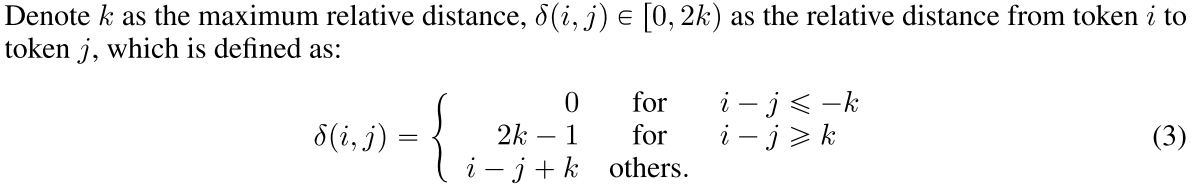
\includegraphics[width=\textwidth]{img/reldist}
\end{figure}

\begin{itemize}
\item the positional vectors are relative = [-2, -1, 0, 1, 2]
\item the positional encodings are shared between layers
\item max relative distance = $k=512$, after that just pad: [-2, -2, -1, 0]
\end{itemize}

\end{frame}
%--------- END Frame 12 -------------
\begin{frame}{Ablation study: everything helps}

\begin{figure}[h]
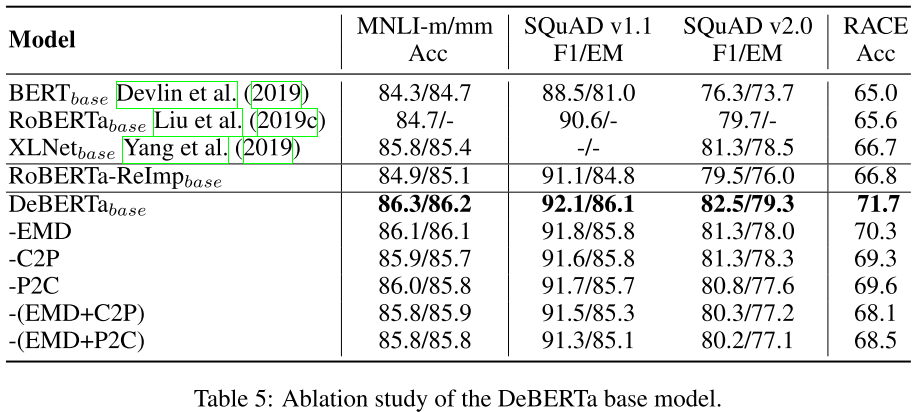
\includegraphics[width=\textwidth]{img/ablation}
\end{figure}

\end{frame}
%--------- END Frame 12 -------------
\begin{frame}{Pre-training needs less steps than RoBERTa}

\begin{figure}[h]
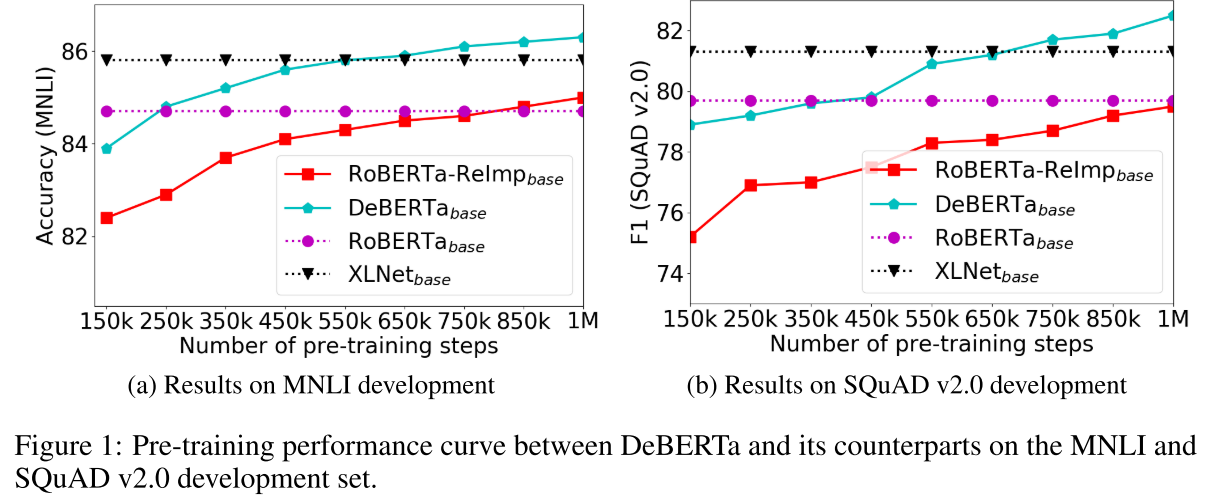
\includegraphics[width=\textwidth]{img/pretraining}
\end{figure}

\end{frame}
%--------- END Frame 12 -------------
\begin{frame}{Sources}
\begin{thebibliography}{0}

  \bibitem[1]{cit:paper} 1.He, Pengcheng, et al. "Deberta: Decoding-enhanced bert with disentangled attention." arXiv preprint arXiv:2006.03654 (2020). \url{https://arxiv.org/abs/2006.03654} 
  
  \bibitem[2]{cit:vae} 2. VAE overview blog post. \url{https://lilianweng.github.io/lil-log/2018/08/12/from-autoencoder-to-beta-vae.html}
  
  \bibitem[3]{snail} 3. Chen, Xi, et al. "Pixelsnail: An improved autoregressive generative model." International Conference on Machine Learning. PMLR, 2018. \url{https://arxiv.org/abs/1712.09763}
  
  \bibitem[4]{dp} 4. Razavi, Ali, Aaron van den Oord, and Oriol Vinyals. "Generating diverse high-fidelity images with vq-vae-2." arXiv preprint arXiv:1906.00446 (2019). \url{https://arxiv.org/abs/1906.00446}
  
  \bibitem[5]{dp} 5. VQ-VAE implementation \url{https://github.com/nadavbh12/VQ-VAE/tree/master/vq_vae}
  
\end{thebibliography}

\end{frame}

 
\end{document}
